\documentclass{beamer}
\usepackage{listings}
\usepackage{hyperref,animate}
\usepackage{tikz}
\usetikzlibrary{positioning,shadows,arrows,shapes,calc}
\def\labelenumi\theenumi
\usepackage{graphicx}
\usepackage{amsmath}
\mode<presentation>{\usetheme{Frankfurt}}
\AtBeginSection
{
  \begin{frame}<beamer>
    \frametitle{Outline}
    \tableofcontents[currentsection,currentsubsection]
  \end{frame}
}
\title{Lecture 23: Recurrent Neural Nets}
\author{Mark Hasegawa-Johnson}
\date{ECE 417: Multimedia Signal Processing}  
\titlegraphic{\includegraphics{../../../17fall/lectures/imark_1867_bold.png}}
\begin{document}

% Title
\begin{frame}
  \maketitle
\end{frame}

% Title
\begin{frame}
  \tableofcontents
\end{frame}

%%%%%%%%%%%%%%%%%%%%%%%%%%%%%%%%%%%%%%%%%%%%%%%%%%%%%%%%%
\section[CNN/RNN]{Nonlinear Time Invariant Filtering: CNN \& RNN}
\setcounter{subsection}{1}

\begin{frame}
  \frametitle{Convolutional Neural Net = Nonlinear(FIR)}
  \centerline{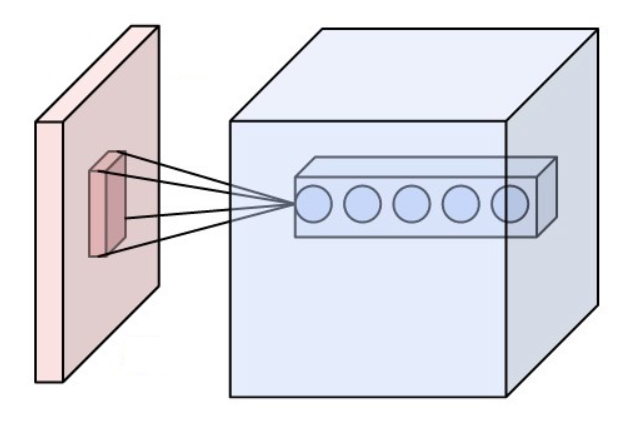
\includegraphics[height=1.5in]{exp/Conv_layer.png}}
  \begin{tiny}Image CC-SA-4.0  by Aphex34, \url{https://commons.wikimedia.org/wiki/File:Conv_layer.png}\end{tiny}
\end{frame}

\begin{frame}
  \frametitle{Convolutional Neural Net = Nonlinear(FIR)}
  \[
  h[n] = \sigma\left(\sum_{m=0}^{N-1}w[m]x[n-m]\right)
  \]
  The coefficients, $w[m]$, are chosen to minimize some kind of loss
  function.  For example, suppose that the goal is to make $h[n]$
  resemble a target signal $y[n]$; then we might use
  \[
  {\mathcal L} = \frac{1}{2}\sum_{n=0}^N\left(h[n]-y[n]\right)^2
  \]
  and choose
  \[
  w[n] \leftarrow w[n]-\eta\frac{d{\mathcal L}}{dw[n]}
  \]
\end{frame}

\begin{frame}
  \frametitle{Recurrent Neural Net (RNN) = Nonlinear(IIR)}
  \centerline{\includegraphics[width=4.5in]{exp/800px-Recurrent_neural_network_unfold.svg.png}}
  \begin{tiny}Image CC-SA-4.0  by Ixnay, \url{https://commons.wikimedia.org/wiki/File:Recurrent_neural_network_unfold.svg}\end{tiny}
\end{frame}

\begin{frame}
  \frametitle{Recurrent Neural Net (RNN) = Nonlinear(IIR)}
  \[
  h[n] = \sigma\left(x[n] + \sum_{m=1}^{M-1}w[m] h[n-m]\right)
  \]
  The coefficients, $w[m]$, are chosen to minimize the loss function.
  For example, suppose that the goal is to make $h[n]$ resemble a
  target signal $y[n]$; then we might use 
  \[
  {\mathcal L} = \frac{1}{2}\sum_{n=0}^N\left(h[n]-y[n]\right)^2
  \]
  and choose
  \[
  w[m] \leftarrow w[m]-\eta\frac{d{\mathcal L}}{dw[m]}
  \]
\end{frame}

%%%%%%%%%%%%%%%%%%%%%%%%%%%%%%%%%%%%%%%%%%%%%%%%%%%%%%%%%
\section[Back-Prop]{Back-Propagation Review}
\setcounter{subsection}{1}

\begin{frame}
  \frametitle{Flow Graphs}

  \centerline{
    \tikzstyle{pre}=[<-,shorten <=1pt,>=stealth',semithick,draw=blue]
    \begin{tikzpicture}[hoop/.style={circle,thick,draw=blue,text=black,
          fill=orange!35!white,text centered,text width=0.25cm}]
      \node[hoop] (x) at (0,0) {$x$};
      \node[hoop] (h0) at (-2,1) {$h_0$} edge[pre] (x);
      \node[hoop] (h1) at (2,2) {$h_1$} edge[pre] (x) edge[pre](h0);
      \node[hoop] (yhat) at (0,3) {$\hat{y}$} edge[pre](h0) edge[pre](h1);
  \end{tikzpicture}}

  Forward propagation can be summarized by a {\bf flow graph}, which
  specifies the dependencies among variables, without specifying the
  functional form of the dependence.  For example, the above graph shows that
  \begin{itemize}
  \item $\hat{y}$ is a function of $h_0$ and $h_1$.
  \item $h_1$ is a function of $x$ and $h_0$.
  \item $h_0$ is a function of $x$.
  \end{itemize}
\end{frame}

\begin{frame}
  \frametitle{Review: Partial and Total Derivatives}
  \begin{itemize}
  \item The {\bf total derivative} symbol, $\frac{d{\mathcal
      L}}{dh_k}$, {\bf always means the same thing}: derivative
    including the contributions of all paths from $h_k$ to ${\mathcal
      L}$.
  \item The {\bf partial derivative} symbol, $\frac{\partial{\mathcal
      L}}{\partial h_k}$, can mean {\bf different things in different
    equations} (because different equations might hold constant a
    different set of other variables).
  \item There is a notation we can use to specify {\bf which} other
    variables are being held constant: $\frac{\partial{\mathcal
        L}}{\partial
      h_k}(\hat{y}_1,\hat{y}_6,\hat{y}_{10},h_1,\ldots,h_N)$ means
    ``hold $\hat{y}_1,\hat{y}_6,\hat{y}_{10},$ and
    $h_1,\ldots,h_{k-1},h_{k+1},\ldots,h_N$ constant.''
  \end{itemize}
\end{frame}

\begin{frame}
  \frametitle{Back-Propagation in terms of Flow Graphs}

  \centerline{
    \tikzstyle{pre}=[<-,shorten <=1pt,>=stealth',semithick,draw=blue]
    \begin{tikzpicture}[hoop/.style={circle,thick,draw=blue,text=black,
          fill=orange!35!white,text centered,text width=0.25cm}]
      \node[hoop] (x) at (0,0) {$x$};
      \node[hoop] (h0) at (-2,1) {$h_0$} edge[pre] (x);
      \node[hoop] (h1) at (2,2) {$h_1$} edge[pre] (x) edge[pre](h0);
      \draw[dashed] (-2.5,1.5) -- (3.5,1.5);
      \node[hoop] (yhat) at (0,3) {$\hat{y}$} edge[pre](h0) edge[pre](h1) edge[pre](x);
  \end{tikzpicture}}

  In order to find the derivative of an output w.r.t. any intermediate variables,
  one strategy that works is:
  \begin{enumerate}
  \item Draw a dashed line across the graph just downstream of the desired intermediate variables.
  \item Apply the chain rule, with a summation across all edges that cross the dashed line.
  \end{enumerate}
\end{frame}

\begin{frame}
  \frametitle{Back-Propagation in terms of Flow Graphs}

  \centerline{
    \tikzstyle{pre}=[<-,shorten <=1pt,>=stealth',semithick,draw=blue]
    \begin{tikzpicture}[hoop/.style={circle,thick,draw=blue,text=black,
          fill=orange!35!white,text centered,text width=0.25cm}]
      \node[hoop] (x) at (0,0) {$x$};
      \node[hoop] (h0) at (-2,1) {$h_0$} edge[pre] (x);
      \node[hoop] (h1) at (2,2) {$h_1$} edge[pre] (x) edge[pre](h0);
      \draw[dashed] (-2.5,1.5) -- (3.5,1.5);
      \node[hoop] (yhat) at (0,3) {$\hat{y}$} edge[pre](h0) edge[pre](h1) edge[pre](x);
  \end{tikzpicture}}

  \begin{align*}
    \frac{\partial\hat{y}}{\partial h_0}(x,h_0) &=
    \frac{d\hat{y}}{dh_1}\frac{\partial h_1}{\partial h_0}(x,h_0,h_1) +
    \frac{d\hat{y}}{d\hat{y}}\frac{\partial\hat{y}}{\partial h_0}(x,h_0,h_1)\\
    \frac{\partial\hat{y}}{\partial x}(x,h_0) &=
    \frac{d\hat{y}}{dh_1}\frac{\partial h_1}{\partial x}(x,h_0,h_1) +
    \frac{d\hat{y}}{d\hat{y}}\frac{\partial\hat{y}}{\partial x}(x,h_0,h_1)
  \end{align*}
  Notice: $\frac{\partial\hat{y}}{\partial x}(x,h_0)$ does {\bf not}
  include $\frac{d\hat{y}}{dh_0}\frac{\partial h_0}{\partial x}$.
\end{frame}

\begin{frame}
  \begin{columns}
    \begin{column}{0.5\textwidth}
      \begin{block}{Fully-Connected Network}
        \begin{center}
          \tikzstyle{pre}=[<-,shorten <=1pt,>=stealth',semithick,draw=blue]
          \tikzstyle{post}=[->,shorten >=1pt,>=stealth',semithick,draw=blue]
          \begin{tikzpicture}[
              hoop/.style={circle,thick, draw=blue, text=black, fill=orange!35!white, text centered, text width=0.25cm},
              open/.style={circle,thick, draw=blue, text=black, text centered, text width=0.25cm}
            ]
            \node (x0) at (0,0) {$1$};
            \node[open] (x1) at (1,0) {$x_1$};
            \node[open] (x2) at (2,0) {$x_2$};
            \node (x3) at (3,0) {\ldots};
            \node[open] (xp) at (4,0) {$x_D$};
            \node (h0) at (0,1.5) {$1$};
            \node[hoop] (h1) at (1,1.5) {$h_1$} edge[pre](x0) edge[pre](x1) edge[pre](xp);
            \node[hoop] (h2) at (2,1.5) {$h_2$} edge[pre](x0) edge[pre](x1) edge[pre](xp);
            \node (y3) at (3,1.5) {\ldots};
            \node[hoop] (hq) at (4,1.5) {$h_N$} edge[pre](x0) edge[pre](x1) edge[pre](xp);
            \node[hoop] (y1) at (1,3) {$\hat{y}_1$} edge[pre](h0) edge[pre](h1) edge[pre](hq);
            \node[hoop] (y2) at (2,3) {$\hat{y}_2$} edge[pre](h0) edge[pre](h1) edge[pre](hq);
            \node (y3) at (3,3) {\ldots};
            \node[hoop] (yr) at (4,3) {$\hat{y}_K$} edge[pre](h0) edge[pre](h1) edge[pre](hq);
            \node (zeta1) at (1,3.75) {} edge[pre](y1);
            \node (zeta2) at (2,3.75) {} edge[pre](y2);
            \node (zetar) at (4,3.75) {} edge[pre](yr);
            \node (output) at (2.5,4) {$\hat{y}=h(\vec{x},W^{(1)},\vec{b}^{(1)},W^{(2)},\vec{b}^{(2)})$};
            \draw[dashed] (0,2.25) -- (5,2.25);
          \end{tikzpicture}
        \end{center}
      \end{block}
    \end{column}
    \begin{column}{0.5\textwidth}
      \begin{block}{Back-Prop in a Fully-Connected Network}
        \begin{displaymath}
          \frac{\partial{\mathcal L}}{\partial h_j}=
          \sum_{k=1}^K\frac{d{\mathcal L}}{d\hat{y}_k}\frac{\partial\hat{y}_k}{\partial h_j}
        \end{displaymath}
      \end{block}
    \end{column}
  \end{columns}
\end{frame}


\begin{frame}
  \begin{columns}
    \begin{column}{0.5\textwidth}
      \begin{block}{Fully-Connected Network}
        \begin{center}
          \tikzstyle{pre}=[<-,shorten <=1pt,>=stealth',semithick,draw=blue]
          \tikzstyle{post}=[->,shorten >=1pt,>=stealth',semithick,draw=blue]
          \begin{tikzpicture}[
              hoop/.style={circle,thick, draw=blue, text=black, fill=orange!35!white, text centered, text width=0.25cm},
              open/.style={circle,thick, draw=blue, text=black, text centered, text width=0.25cm}
            ]
            \node (x0) at (0,0) {$1$};
            \node[open] (x1) at (1,0) {$x_1$};
            \node[open] (x2) at (2,0) {$x_2$};
            \node (x3) at (3,0) {\ldots};
            \node[open] (xp) at (4,0) {$x_D$};
            \node (h0) at (0,1.5) {$1$};
            \node[hoop] (h1) at (1,1.5) {$h_1$} edge[pre](x0) edge[pre](x1) edge[pre](xp);
            \node[hoop] (h2) at (2,1.5) {$h_2$} edge[pre](x0) edge[pre](x1) edge[pre](xp);
            \node (y3) at (3,1.5) {\ldots};
            \node[hoop] (hq) at (4,1.5) {$h_N$} edge[pre](x0) edge[pre](x1) edge[pre](xp);
            \node[hoop] (y1) at (1,3) {$\hat{y}_1$} edge[pre](h0) edge[pre](h1) edge[pre](hq);
            \node[hoop] (y2) at (2,3) {$\hat{y}_2$} edge[pre](h0) edge[pre](h1) edge[pre](hq);
            \node (y3) at (3,3) {\ldots};
            \node[hoop] (yr) at (4,3) {$\hat{y}_K$} edge[pre](h0) edge[pre](h1) edge[pre](hq);
            \node (zeta1) at (1,3.75) {} edge[pre](y1);
            \node (zeta2) at (2,3.75) {} edge[pre](y2);
            \node (zetar) at (4,3.75) {} edge[pre](yr);
            \node (output) at (2.5,4) {$\hat{y}=h(\vec{x},W^{(1)},\vec{b}^{(1)},W^{(2)},\vec{b}^{(2)})$};
            \draw[dashed] (0,0.75) -- (5,0.75);
          \end{tikzpicture}
        \end{center}
      \end{block}
    \end{column}
    \begin{column}{0.5\textwidth}
      \begin{block}{Back-Prop in a Fully-Connected Network}
        \begin{displaymath}
          \frac{\partial{\mathcal L}}{\partial w_{k,j}^{(1)}}=
          \sum_{j=1}^N\frac{d{\mathcal L}}{d h_j}\frac{\partial h_j}{\partial w_{k,j}^{(1)}}
        \end{displaymath}
      \end{block}
    \end{column}
  \end{columns}
\end{frame}


%%%%%%%%%%%%%%%%%%%%%%%%%%%%%%%%%%%%%%%%%%%%%%%%%%%%%%%%%
\section[Back-Prop]{Back-Propagation Training for CNN and RNN}
\setcounter{subsection}{1}

\begin{frame}
  \frametitle{Back-Prop in a CNN}
  Suppose we have a convolutional neural net, defined by
  \begin{align*}
    \xi[n] &= \sum_{m=0}^{N-1}w[m]x[n-m]\\
    h[n] &= g\left(\xi[n]\right)
  \end{align*}
  then 
  \begin{align*}
    \frac{\partial{\mathcal L}}{\partial w[m]}
    & =\sum_n \frac{d{\mathcal L}}{d\xi[n]} \frac{\partial\xi[n]}{\partial w[m]}\\
    & =\sum_n \frac{d{\mathcal L}}{d\xi[n]} x[n-m]\\
  \end{align*}
\end{frame}

\begin{frame}
  \frametitle{Back-Prop in an RNN}
  Suppose we have a recurrent neural net, defined by
  \begin{align*}
    \xi[n] &= x[n] + \sum_{m=1}^{M-1}w[m]h[n-m]\\
    h[n] &= g\left(\xi[n]\right)
  \end{align*}
  then
  \begin{align*}
    \frac{\partial{\mathcal L}}{\partial w[m]}
    & =\sum_n \frac{d{\mathcal L}}{d\xi[n]} \frac{\partial\xi[n]}{\partial w[m]}\\
    & =\sum_n \frac{d{\mathcal L}}{d\xi[n]} h[n-m]\\
  \end{align*}
\end{frame}

%%%%%%%%%%%%%%%%%%%%%%%%%%%%%%%%%%%%%%%%%%%%%%%%%%%%%%%%%
\section[BPTT]{Back-Prop Through Time}
\setcounter{subsection}{1}

\begin{frame}
  \frametitle{Partial vs. Full Derivatives}

  For example, suppose we want $h[n]$ to be as close as possible to
  some target signal $y[n]$:
  \[
  {\mathcal L} = \frac{1}{2}\sum_n \left(h[n]-y[n]\right)^2
  \]
  Notice that ${\mathcal L}$ depends on $h[n]$ in many different ways:
  \[
  \frac{d{\mathcal L}}{dh[n]}=\frac{\partial {\mathcal L}}{\partial h[n]}+
  \frac{d{\mathcal L}}{dh[n+1]}\frac{\partial h[n+1]}{\partial h[n]}+
  \frac{d{\mathcal L}}{dh[n+2]}\frac{\partial h[n+2]}{\partial h[n]}+\ldots
  \]
\end{frame}
\begin{frame}
  \frametitle{Partial vs. Full Derivatives}
  In general,
  \[
  \frac{d{\mathcal L}}{dh[n]}=\frac{\partial {\mathcal L}}{\partial h[n]}+
  \sum_{m=1}^\infty\frac{d{\mathcal L}}{dh[n+m]}\frac{\partial h[n+m]}{\partial h[n]}
  \]
  where
  \begin{itemize}
    \item $\frac{d{\mathcal L}}{dh[n]}$ is the total derivative, and includes all
      of the different ways in which ${\mathcal L}$ depends on $h[n]$.
    \item $\frac{\partial h[n+m]}{\partial h[n]}$ is the partial
      derivative, i.e., the change in $h[n+m]$ per unit change in
      $h[n]$ if $\{h[n+1],\ldots,h[n+m-1]\}$ are all held constant.
  \end{itemize}
\end{frame}

\begin{frame}
  \begin{center}
    \tikzstyle{pre}=[<-,shorten <=1pt,>=stealth',semithick,draw=blue]
    \tikzstyle{post}=[->,shorten >=1pt,>=stealth',semithick,draw=blue]
    \begin{tikzpicture}[
        hoop/.style={circle,thick, draw=blue, text=black, fill=orange!35!white, text centered, text width=0.75cm},
        open/.style={circle,thick, draw=blue, text=black, text centered, text width=0.75cm}
      ]
      \node[open] (x0) at (-2,0) {$x[0]$};
      \node (x1) at (0,0) {\ldots};
      \node[open] (xn) at (2,0) {$x[n]$};
      \node[open] (xn1) at (4,0) {\tiny $x[n+1]$};
      \node (x3) at (6,0) {\ldots};
      \node[open] (xT) at (8,0) {$x[T]$};
      \node[hoop] (h0) at (-2,1.5) {$h[0]$} edge[pre](x0);
      \node (h1) at (0,1.5) {\ldots} edge[pre](h0);
      \node[hoop] (hn) at (2,1.5) {$h[n]$} edge[pre](xn) edge[pre](h1);
      \node[hoop] (hn1) at (4,1.5) {\tiny $h[n+1]$} edge[pre](xn1) edge[pre,in=30,out=150](h0) edge[pre](hn);
      \node (h3) at (6,1.5) {\ldots} edge[pre](hn1);
      \node[hoop] (hT) at (8,1.5) {$h[T]$} edge[pre](xT) edge[pre,in=30,out=150](h0)
      edge[pre,in=30,out=150](hn)  edge[pre](h3);
      \node[hoop] (L) at (8,3.5) {$\mathcal L$} edge[pre](hT) edge[pre](h0) edge[pre](hn)  edge[pre](hn1);
    \end{tikzpicture}
  \end{center}
  Here's a flow diagram that could represent:
  \begin{align*}
    h[n] &= g\left(x[n]+\sum_{m=0}^\infty w[m]h[n-m]\right)\\
    {\mathcal L} &= \frac{1}{2}\sum_n (y[n]-h[n])^2
  \end{align*}
\end{frame}

\begin{frame}
  \begin{center}
    \tikzstyle{pre}=[<-,shorten <=1pt,>=stealth',semithick,draw=blue]
    \tikzstyle{post}=[->,shorten >=1pt,>=stealth',semithick,draw=blue]
    \begin{tikzpicture}[
        hoop/.style={circle,thick, draw=blue, text=black, fill=orange!35!white, text centered, text width=0.75cm},
        open/.style={circle,thick, draw=blue, text=black, text centered, text width=0.75cm}
      ]
      \node[open] (x0) at (-2,0) {$x[0]$};
      \node (x1) at (0,0) {\ldots};
      \node[open] (xn) at (2,0) {$x[n]$};
      \node[open] (xn1) at (4,0) {\tiny $x[n+1]$};
      \node (x3) at (6,0) {\ldots};
      \node[open] (xT) at (8,0) {$x[T]$};
      \node[hoop] (h0) at (-2,1.5) {$h[0]$} edge[pre](x0);
      \node (h1) at (0,1.5) {\ldots} edge[pre](h0);
      \node[hoop] (hn) at (2,1.5) {$h[n]$} edge[pre](xn) edge[pre](h1);
      \node[hoop] (hn1) at (4,1.5) {\tiny $h[n+1]$} edge[pre](xn1) edge[pre,in=30,out=150](h0) edge[pre](hn);
      \node (h3) at (6,1.5) {\ldots} edge[pre](hn1);
      \node[hoop] (hT) at (8,1.5) {$h[T]$} edge[pre](xT) edge[pre,in=30,out=150](h0)
      edge[pre,in=30,out=150](hn)  edge[pre](h3);
      \node[hoop] (L) at (8,3.5) {$\mathcal L$} edge[pre](hT) edge[pre](h0) edge[pre](hn)  edge[pre](hn1);
      \draw[dashed] (3,-0.5) -- (3,4);
    \end{tikzpicture}
  \end{center}
  Back-propagation through time does this:
  \begin{align*}
    \frac{d{\mathcal L}}{dh[n]}
    &=\frac{\partial {\mathcal L}}{\partial h[n]} +
    \sum_{m=1}^{T-n}\frac{d{\mathcal L}}{dh[n+m]}\frac{\partial h[n+m]}{\partial h[n]}
  \end{align*}
\end{frame}

\begin{frame}
  \frametitle{Partial vs. Full Derivatives}

  So for example, if
  \[
  {\mathcal L} = \frac{1}{2}\sum_n \left(h[n]-y[n]\right)^2
  \]
  then the partial derivative of ${\mathcal L}$ w.r.t. $h[n]$ is 
  \[
  \frac{\partial {\mathcal L}}{\partial h[n]}= h[n]-y[n]
  \]
  and the total derivative of ${\mathcal L}$ w.r.t. $h[n]$ is 
  \[
  \frac{d{\mathcal L}}{dh[n]}=\left(h[n]-y[n]\right)+
  \sum_{m=1}^\infty\frac{d{\mathcal L}}{dh[n+m]}\frac{\partial h[n+m]}{\partial h[n]}
  \]
\end{frame}

\begin{frame}
  \frametitle{Partial vs. Full Derivatives}

  So for example, if
  \[
  h[n] =g(\xi[n]),~~~~\xi[n]=x[n]+\sum_{m=1}^{M}w[m]h[n-m]
  \]
  then the partial derivative of $h[n+k]$ w.r.t. $h[n]$ is 
  \[
  \frac{\partial h[n+k]}{\partial h[n]}= \dot{g}(\xi[n+k]) w[k] 
  \]
  where we use the notation $\dot{g}(\xi)=\frac{dg}{d\xi}$.
\end{frame}

\begin{frame}
  \frametitle{Synchronous Backprop vs. BPTT}

  The basic idea of back-prop-through-time is divide-and-conquer.
  \begin{enumerate}
    \item {\bf Synchronous Backprop:} First, calculate the {\bf\em
      partial derivative} of ${\mathcal L}$ w.r.t. the excitation $\xi[n]$ at time
      $n$, assuming that all other time steps are held constant.
      \[
      \epsilon[n] = \frac{\partial {\mathcal L}}{\partial\xi[n]}
      \]
    \item {\bf Back-prop through time:} Second, iterate backward
      through time to calculate the {\bf\em total derivative}
      \[
      \delta[n] = \frac{d{\mathcal L}}{d\xi[n]}
      \]
  \end{enumerate}
\end{frame}

\begin{frame}
  \frametitle{Synchronous Backprop in an RNN}
  Suppose we have a recurrent neural net, defined by
  \begin{align*}
    \xi[n] &= x[n] + \sum_{m=1}^{M}w[m] h[n-m]\\
    h[n] &= g\left(\xi[n]\right)\\
    {\mathcal L} &= \frac{1}{2}\sum_n\left(h[n]-y[n]\right)^2
  \end{align*}
  then
  \[
  \frac{\partial {\mathcal L}}{\partial h[n]} = \left(h[n]-y[n]\right)
  \]
\end{frame}
  
\begin{frame}
  \frametitle{Back-Prop Through Time (BPTT)}
  Suppose we have a recurrent neural net, defined by
  \begin{align*}
    \xi[n] &= x[n] + \sum_{m=1}^{M}w[m] h[n-m]\\
    h[n] &= g\left(\xi[n]\right)\\
    {\mathcal L} &= \frac{1}{2}\sum_n\left(h[n]-y[n]\right)^2
  \end{align*}
  then
  \begin{align*}
    \frac{d{\mathcal L}}{d h[n]}
    &=\frac{\partial {\mathcal L}}{\partial h[n]}+
    \sum_{m=1}^{\infty}\frac{d{\mathcal L}}{d h[n+m]}\frac{\partial h[n+m]}{\partial h[n]}\\
    &=\frac{\partial {\mathcal L}}{\partial h[n]}+
    \sum_{m=1}^{M}\frac{d{\mathcal L}}{d\xi[n+m]}\dot{g}(\xi[n+m]) w[m]
  \end{align*}
\end{frame}
  
\begin{frame}
  \frametitle{Weight Gradient}
  Suppose we have a recurrent neural net, defined by
  \begin{align*}
    \xi[n] &= x[n] + \sum_{m=1}^{M}w[m] h[n-m]\\
    h[n] &= g\left(\xi[n]\right)\\
    {\mathcal L} &= \frac{1}{2}\sum_n\left(h[n]-y[n]\right)^2
  \end{align*}
  then the weight gradient is given by
  \begin{align*}
    \frac{\partial{\mathcal L}}{\partial w[m]}\left(w[1],\ldots,w[M]\right)
    &=\sum_{n}\frac{d{\mathcal L}}{d h[n]}\frac{\partial h[n]}{\partial w[m]}\left(w[1],\ldots,w[M]\right)\\
    &=\sum_{n}\frac{d{\mathcal L}}{dh[n]}\dot{g}(\xi[n]) h[n-m]
  \end{align*}
\end{frame}
  
%%%%%%%%%%%%%%%%%%%%%%%%%%%%%%%%%%%%%%%%%%%%%%%%%%%%%%%%%%%%%%%%%%%%%%%%%%%%%%%%%
\section{Conclusion}
\setcounter{subsection}{1}

\begin{frame}
  \frametitle{Conclusions}
  \begin{itemize}
  \item Back-Prop, in general, is just the chain rule of calculus:
    \begin{displaymath}
      \frac{d{\mathcal L}}{dw} = \sum_{i=0}^{N-1}\frac{d{\mathcal L}}{dh_i}\frac{\partial h_i}{\partial w}
    \end{displaymath}
  \item Convolutional Neural Networks are the nonlinear version of an FIR filter.
    Coefficients are shared across time steps.
  \item Recurrent Neural Networks are the nonlinear version of an IIR filter.  
    Coefficients are shared across time steps.
    Error is back-propagated from every output time step to every input time step.
    \begin{displaymath}
      \frac{d{\mathcal L}}{dh[n]}
      =\frac{\partial {\mathcal L}}{\partial h[n]}+
      \sum_{m=1}^{M}\frac{d{\mathcal L}}{dh[n+m]}\dot{g}(\xi[n+m])w[m]
    \end{displaymath}
    \begin{align*}
      \frac{\partial{\mathcal L}}{\partial w[m]}\left(w[1],\ldots,w[M]\right)
      &=\sum_{n}\frac{d{\mathcal L}}{dh[n]}\dot{g}(\xi[n]) h[n-m]
    \end{align*}
  \end{itemize}
\end{frame}

%%%%%%%%%%%%%%%%%%%%%%%%%%%%%%%%%%%%%%%%%%%%%%%%%%%%%%%%%%%%%%%%%%%%%%%%%%%%%%%%%
\section[Example]{Written Example}
\setcounter{subsection}{1}

\begin{frame}
  \frametitle{Written Example}
  Suppose that $\vec{h}[t]=[h_1[t],\ldots,h_N[t]]^T$ is a vector, and suppose that
  \begin{align*}
    \vec{h}[t] &= \mbox{tanh}\left(U\vec{x}[t] + V_1\vec{h}[t-1]+V_2\vec{h}[t-2]\right)\\
        {\mathcal L} &= \frac{1}{2}\sum_t \Vert\vec{y}-W\vec{h}[t]\Vert^2
  \end{align*}
  where $U$ is a $N\times D$ matrix, $W$ is a $K\times N$ matrix, and
  $V_1$ and $V_2$ are $N\times N$ matrices.  Find an algorithm to
  compute $\nabla_{\vec{h}[t]}{\mathcal L}$.
\end{frame}


\end{document}

